\section{Experimentación}
    En esta sección, se presentan las pruebas experimentales realizadas sobre ambas implementaciones de los algoritmos, como así también los resultados obtenidos en cada una de ellas y una discusión de los mismos. El objetivo detrás de la realización de estos experimentos fue evaluar y comparar el rendimiento de las diferentes implementaciones, para extraer conclusiones acerca de las características del modelo de programación \acr{SIMD}.

    Todas las pruebas, como así también los gráficos que se incluyen en este informe, pueden ser recreadas mediante la ejecución de una serie de \emph{scripts} incluidos con los archivos fuentes del trabajo práctico. Estos \emph{scripts}, programados en Bash, se encuentran en el directorio \texttt{exp}, y llevan por nombre \texttt{exp\{i\}}, donde \texttt{i} es el número del experimento. El parámetro opcional \texttt{-n <cant>} permite elegir la cantidad de veces que se repetirá cada medición.

    \subsection{Experimento 1: Comparación de rendimiento}

        \subsubsection*{Presentación}
        	En este experimento, se buscó comparar el rendimiento de las implementaciones en lenguaje C de ambos filtros, con el obtenido con las respectivas implementaciones en lenguaje ensamblador utilizando el paradigma \acr{SIMD}. Las pruebas se realizaron con diferentes tamaños de imágenes, con el objetivo de lograr una comparación independiente de dicho parámetro y, al mismo tiempo, adquirir una idea del comportamiento empírico de cada implementación con respecto al tamaño de la entrada.

        \subsubsection*{Metodología, datos y parámetros del experimento}
        	El experimento consistió en la aplicación de las dos implementaciones de ambos filtros a una serie de imágenes de diferentes tamaños; en todos los casos se midió el tiempo de ejecución, utilizando la instrucción \texttt{RDTSC} de la arquitectura \emph{x86-64}. Para mejorar la calidad de los resultados cada medición se repitió un total de 20 veces, calculando luego el tiempo promedio insumido por iteración.

        	Como dato de entrada, se consideró una imagen de $1800 \times 1200$ píxeles ($2160000$ píxeles en total), que puede encontrarse bajo el nombre \texttt{img/phoebe1.bmp}; para utilizar con el filtro \emph{diff}, además, se utilizó una versión modificada de la misma, \texttt{img/phoebe2.bmp}. Redimensionando ambas imágenes se crearon versiones de los siguientes tamaños en píxeles: \{1801824, 1500000, 1024224, 960000, 726624, 540000, 369024, 240000, 1536000, 60000, 38400, 21600, 9600, 6144, 2400, 1536, 864, 384\}.

        	Por otra parte, como parámetros del filtro \emph{blur} se seleccionaron arbitrariamente los valores $\sigma = 5$ y $r = 15$, manteniendo los mismos constantes a lo largo de todo el experimento.

        \subsubsection*{Hipótesis}
            Se espera observar que la implementación en lenguaje ensamblador de ambos filtros sea más eficiente, independientemente del tamaño de la imagen. Esto se debe a que hacen uso del modelo \acr{SIMD}, con todas las ventajas ya mencionadas que esto tiene sobre el rendimiento del código, a diferencia de las implementaciones de los algoritmos en C, que procesan cada píxel de manera independiente. Esto último puede inferirse no solo de la estructura propia del código, cuyos ciclos iteran sobre un único píxel a la vez, sino también de la ausencia de instrucciones \acr{SEE} para procesamiento de valores empaquetados que se observa al desensamblar los objetos compilados a partir de este código.

        \subsubsection*{Resultados obtenidos y discusión}

            \noindent{} \begin{minipage}{\textwidth}
                \begin{center}
                    \vspace{1em}
                    \begin{tabular}{cc}
                        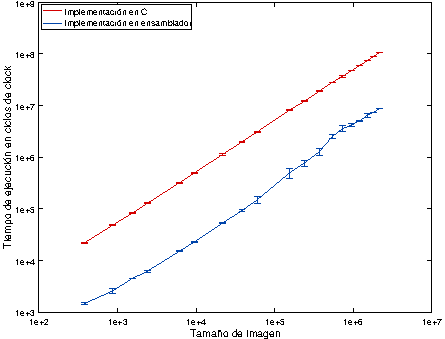
\includegraphics{graficos/exp1-diff-c_vs_asm.pdf} & 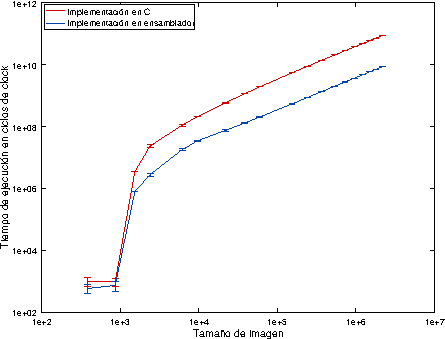
\includegraphics{graficos/exp1-blur-c_vs_asm.pdf} \\
                        {\small Filtro \emph{diff}}                       & {\small Filtro \emph{blur}}
                        \vspace{1em}
                    \end{tabular}
                    Resultados arrojados por el experimento 1. Los gráficos muestran, para ambas implementaciones, el tiempo de ejecución según el tamaño en píxeles de la imagen.
                \end{center}
            \end{minipage}

            \noindent{} \begin{minipage}{\textwidth}
                \begin{center}
                    \vspace{1em}
                    \begin{tabular}{cc}
                        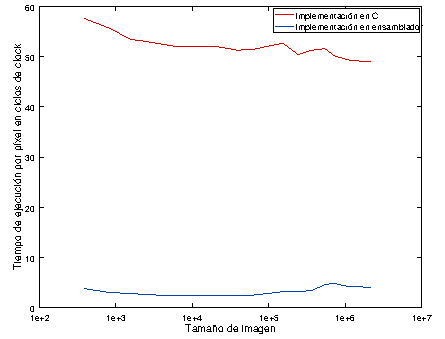
\includegraphics{graficos/exp1-diff-tiempo_por_pixel.pdf} & 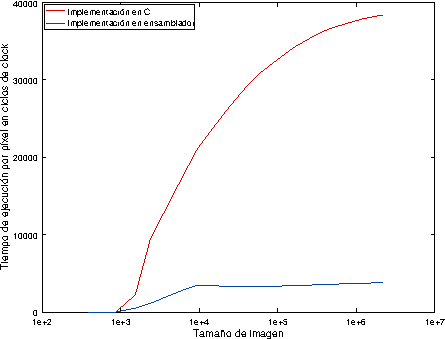
\includegraphics{graficos/exp1-blur-tiempo_por_pixel.pdf} \\
                        {\small Filtro \emph{diff}}                               & {\small Filtro \emph{blur}}
                        \vspace{1em}
                    \end{tabular}
                    Resultados arrojados por el experimento 1. Aquí los resultados se muestran normalizados, mostrando el tiempo insumido por el procesamiento de cada píxel.
                \end{center}
            \end{minipage}

             Como se observa en los resultados, se pudo confirmar la hipótesis planteada: la implementación en lenguaje ensamblador resultó más rápida que la implementación en C para todos los tamaños de imagen.

             En \emph{blur}, cuando llamamos a la función con un valor de $r$ mayor a la mitad de la altura o a la mitad del ancho de la imagen, no se producen cambios. Dado que en el experimento el valor de $r$ se mantiene constante, las dos imágenes más pequeñas no se ven afectadas por el filtro, lo cual se ve reflejado en los resultados, ya que para estas dos imágenes el tiempo de ejecución es notablemente menor.

    \subsection{Experimento 2: Rendimiento según parámetros del filtro \emph{blur}}

        \subsubsection*{Presentación}
            Este experimento se llevó a cabo con el objetivo de analizar el impacto de los diferentes parámetros del filtro \emph{blur} en el rendimiento temporal de ambas implementaciones del mismo.

        \subsubsection*{Metodología, datos y parámetros del experimento}
            Para la realización del experimento se consideró una única imagen de $400 \times 600$ píxeles, es decir, un total de $240000$ píxeles. Luego, se ejecutaron múltiples instancias de ambas implementaciones; esto se hizo en dos etapas, en las que se evaluó por separado el impacto de cada parámetro en el rendimiento general:
            \begin{enumerate}[label=(\alph*)]
                 \item Se mantuvo constante el parámetro $\sigma = 5$, y se varió $r$, tomando los valores \{1, 2, 3, 4, 5, 8, 11, 14, 17, 20, 23, 26, 29, 32, 35, 38\}.
                 \item Se mantuvo constante el parámetro $r = 10$, y se varió $\sigma$, tomando los valores \{0.5, 1, 1.5, 3, 6, 9, 12, 15, 18, 21, 24, 27, 30, 33, 36, 39, 42, 45, 48, 50\}.
             \end{enumerate}

            En cada una de las instancias consideradas, se midió el tiempo de ejecución. Esto se hizo, al igual que en el experimento anterior, mediante la instrucción \texttt{RDTSC} de la arquitectura \emph{x86-64}, repitiendo 20 veces cada medición y calculando luego el tiempo promedio entre estos resultados.
            
        \subsubsection*{Hipótesis}
             Se conjetura que, a medida que el valor del radio $r$ se incrementa, el tiempo de ejecución en las dos implementaciones aumentará, y que lo hará de manera cuadrática con respecto al incremento en $r$. Esto se debe a que la complejidad temporal de cada ejecución del ciclo principal del algoritmo depende del tamaño de la matriz de convolución, que es $(2r + 1) \times (2r + 1) \times 4$, es decir, es cuadrático en el valor de $r$.

             Debido a que el valor del sigma es utilizado solamente para realizar un cálculo por cada posición de la matriz de convolución, se estima que modificar este valor no alterará el tiempo de ejecución.

        \subsubsection*{Resultados obtenidos y discusión}
            \noindent{} \begin{minipage}{\textwidth}
                \begin{center}
                    \vspace{1em}
                    \begin{tabular}{cc}
                        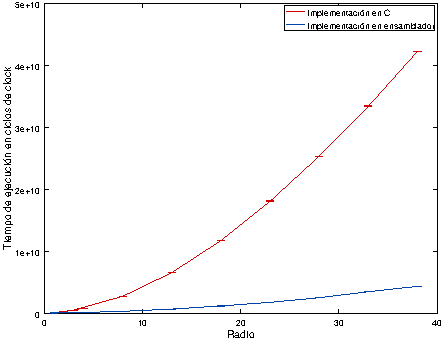
\includegraphics{graficos/exp2-tiempo_segun_radio.pdf} & 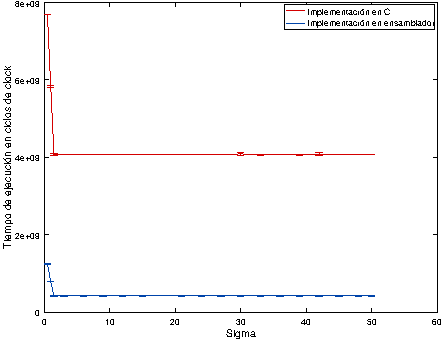
\includegraphics{graficos/exp2-tiempo_segun_sigma.pdf} \\
                        {\small Rendimiento según valor de $r$}                & {\small Rendimiento según valor de $\sigma$}
                        \vspace{1em}
                    \end{tabular}
                    Resultados arrojados por el experimento 2.
                \end{center}
            \end{minipage}

             Se puede observar en los gráficos que a medida que los $r$ aumenta, también lo hace el tiempo de ejecución. En este sentido, se pudo confirmar la hipótesis. Sin embargo, si se dividen los valores del tiempo de ejecución por su correspondiente $r^2$, se comprueba que la relación no es lineal; es decir, el tiempo de ejecución no varía cuadráticamente con el valor de $r$.

            Como se había previsto en la hipótesis, la variación del $\sigma$ no afecta el tiempo de ejecución del algoritmo, tanto en lenguaje ensamblador como en C. Puede observarse que, para valores de $\sigma$ menores que 1, el tiempo de ejecución es notoriamente mayor. Este es un comportamiento inesperado, que sería interesante estudiar posteriormente.

    \subsection{Experimento 3: Peso de llamados a función}

        \subsubsection*{Presentación}
            Al realizar este experimento, se buscó descubrir cuál es el peso que tienen en el rendimiento de los diversos algoritmos los llamados a función. Para este fin se utilizó la técnica de \emph{inlining}, que consiste en tomar el código principal y reemplazar los llamados a función por el mismo código de la función. De esta manera, se buscó evaluar la utilidad y el beneficio de estos llamados a funciones auxiliares. 

        \subsubsection*{Metodología, datos y parámetros del experimento}
            Al igual que en los dos experimentos anteriores, el tiempo de ejecución se tomó utilizando la instrucción \texttt{RDTSC} de la arquitectura \emph{x86-64}, repitiendo 20 veces cada medición y calculando luego el tiempo promedio.
             En particular, se consideraron la versión en lenguaje C de \emph{diff}, a la que se le reemplazaron macros de preprocesador utilizadas para realizar operaciones aritméticas por llamados a función, y la implementación en ensamblador de \emph{blur}, con la que se hizo el proceso opuesto, eliminando los llamados a funciones auxiliares y colocando todo el código directamente en el cuerpo de la función principal.
             En este experimento el ancho de las imágenes utilizadas como parámetro se encuentran en un rango entre 24 y 1800 píxeles. Además, para el filtro \emph{blur}, se utilizó $r = 15$ y $\sigma = 5$.

        \subsubsection*{Hipótesis}
             Creemos que la versión del código implementada que no realiza llamados a funciones va a tener un mejor rendimiento, ya que se evita el overhead que producen estos llamados.

        \subsubsection*{Resultados obtenidos y discusión}

            \noindent{} \begin{minipage}{\textwidth}
                \begin{center}
                    \vspace{1em}
                    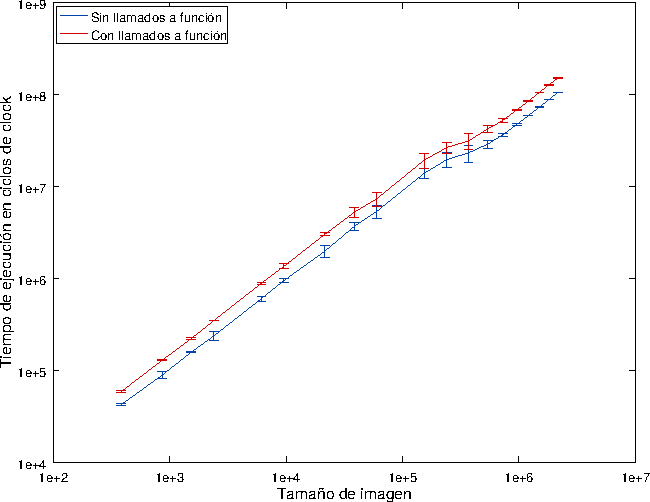
\includegraphics{graficos/exp3-diff-c_vs_c2.pdf}
                    \vspace{1em}

                    Resultados arrojados por el experimento 3. Comparación entre el rendimiento de \emph{diff} en C con y sin llamadas a función.
                \end{center}
            \end{minipage}

            \noindent{} \begin{minipage}{\textwidth}
                \begin{center}
                    \vspace{1em}
                    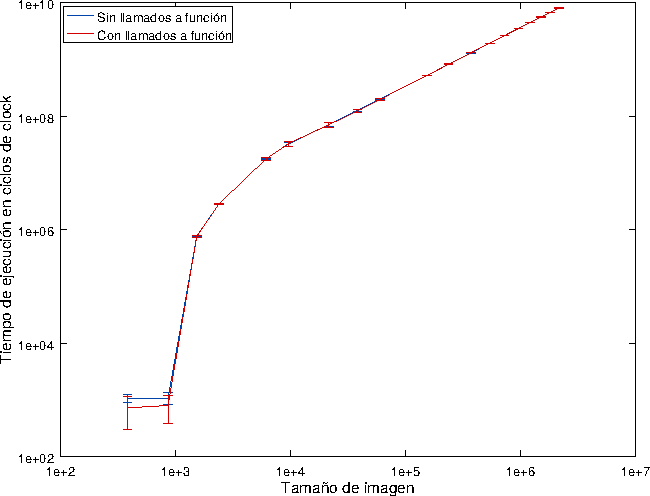
\includegraphics{graficos/exp3-blur-asm_vs_asm2.pdf}
                    \vspace{1em}

                    Resultados arrojados por el experimento 3. Comparación entre el rendimiento de \emph{blur} en ensamblador con y sin llamadas a función.
                \end{center}
            \end{minipage}

            Como muestran los gráficos de la implementación en C, los algoritmos que hacen llamados a otras funciones tienen un mayor tiempo de ejecución que las que no los hacen. Esto se debe a que cada vez que se hace un llamado a función, en necesario modificar la pila, manteniéndola alineada y guardando los registros que se deben preservar según la convención C y fueron utilizados a lo largo de la función.

            En lenguaje ensamblador, cuando implementamos el algoritmo sin el llamado a la función auxiliar, sigue siendo necesario acceder a la pila ya que hay que reutilizar registros que se tienen que mantener para la convención C. Estos registros son R11 y R13. Eliminarlos implicaría que los cálculos necesarios para poder realizar el filtro no se puedan llevar a cabo. Por esto, seguimos haciendo accesos a memoria. Una vez que la accedemos es muy posible que en la caché se encuentren los siguientes accesos a realizar. Entonces, la diferencia entre accederla pocas veces o algunas más es muy pequeña, ya que el acceso a memoria caché no es muy caro.

            Posiblemente, si se reformulara por completo la estructura del algoritmo y la manera en que se utilizan los registros, podría lograrse una implementación en lenguaje ensamblador que saque una ventaja más considerable. Sin embargo, esto representaría una labor muy costosa, y hay que tener en cuenta que un código que no realiza llamadas a funciones auxiliares es más difícil de mantener y menos legible, por lo que la ganancia obtenida en rendimiento sería probablemente muy pequeña en relación con las desventajas que se ocasionarían.